\documentclass[11pt,a4paper]{article}
%--------------------------------------------------
%Packages bases
\usepackage{lmodern}
\usepackage[spanish]{babel}
\usepackage[utf8]{inputenc}
\usepackage{array}
\usepackage{ifthen}
\usepackage{transparent}
\usepackage{eso-pic}
\usepackage{multirow}
\usepackage{afterpage}
\usepackage{amsfonts}
\usepackage{amssymb}
\usepackage{amsthm}
\usepackage{float}
\usepackage{ifthen}
\usepackage{framed}
\usepackage{xspace}
\usepackage{multicol}
\usepackage{enumitem}
\usepackage{color}
\usepackage{titlesec}
\usepackage{ifthen}


%----------------------------------------
%design
\usepackage{amsmath,tikz}
\usepackage{verbatim}
\usetikzlibrary{shapes.geometric}
\usetikzlibrary{arrows}

%----------------------------------------
%color
\usepackage{transparent}
\usepackage{colortbl}
\definecolor{darkred}{rgb}{.7,0.03,0.22}
\definecolor{red_tab}{rgb}{0.96,0.88,0.86}
\definecolor{darkblue}{HTML}{0000CC}
\definecolor{vdarkblue}{HTML}{000066}
\definecolor{texte}{HTML}{660099}
\definecolor{comt}{HTML}{009933}
%-----------------------------------------


%------------------------------------------
%counters
\newcounter{step}
\newcounter{substep}
\setcounter{step}{0}
\setcounter{substep}{0}
%------------------------------------------

\usepackage{tabularx}
\usepackage{makecell}


\newcolumntype{R}[1]{>{\raggedleft\arraybackslash }p{#1}}
\newcolumntype{L}[1]{>{\raggedright\arraybackslash }p{#1}}
\newcolumntype{C}[1]{>{\centering\arraybackslash }p{#1}}

\usepackage{wasysym}


\usepackage{ifluatex}
\ifluatex
\usepackage{fontspec}
\usepackage{polyglossia}
\setdefaultlanguage{french}
\else
\usepackage[utf8]{inputenc}
\usepackage[T1]{fontenc}
\usepackage{babel}


%-----------------------------------------
%format page
\usepackage[a4paper,left=2cm,right=1cm,top=0.5cm,bottom=1cm,headheight=0cm, headsep=0cm, footskip=0cm,includefoot,includehead]{geometry}

%----------------------------------------
%footnote and header number
\usepackage{fancyhdr}
\usepackage[pages=all]{background}
\pagestyle{fancy}
\renewcommand{\headrulewidth}{0pt}
\fancyhf {} % clear all headers and footers

% Header is used to include the page background
\backgroundsetup{
scale=1,
color=black,
opacity=1,
angle=0,
contents={%
  
\includegraphics[width=\paperwidth,height=\paperheight]{images/paper.jpg}
  }%
}

%-----------------------------------------
%Hyperlink
\usepackage[colorlinks, bookmarks, linkcolor=black, citecolor=black, urlcolor=blue]{hyperref}

%-----------------------------------------
%Set Monospace font
% \usepackage{everysel}
%     \renewcommand*\familydefault{\ttdefault}
%     \EverySelectfont{%
%     \fontdimen2\font=0.4em  % interword space
%     \fontdimen3\font=0.2em  % interword stretch
%     \fontdimen4\font=0.1em  % interword shrink
%     \fontdimen7\font=0.1em  % extra space
%     \hyphenchar\font=`\-    % to allow hyphenation
% }
%-----------------------------------------
%Configurations
\newcommand{\Style}[1]{
\ifthenelse{#1=1}{\makeatletter
\newcommand{\PrepTime}[1]{\def\@PrepTime{#1\xspace}
\def\PrepTimeb{#1}}
\newcommand{\CookingTime}[1]{\def\@CookingTime{#1\xspace}}
\newcommand{\background}[1]{%
\AddToShipoutPictureBG{\AtPageLowerLeft{\transparent{0.1}\includegraphics[width=\paperwidth,height=\paperheight]{#1}}}
}
\newcommand{\CookingTempe}[1]{%
\ifnum0=#1\relax
   \def\@CookingTempe{} 
\else
  \def\@CookingTempe{-- #1$^{\circ}$} 
\fi
}

\newcommand{\TypeCooking}[1]{\def\@TypeCooking{#1}}
\newcommand{\NPerson}[1]{\def\@NbPerson{#1\xspace}}
\newcommand{\Image}[2]{\def\@ImageDim{#1} \def\@ImagePath{#2}}
\def\maketitle{%

\vspace*{0.05cm}
\begin{center}
{\Huge \@title}
\end{center}
}

\newenvironment{ingredient}
  {\noindent\begingroup\edef\x{\endgroup\noexpand}\x
  \maketitle
  
  \begin{footnotesize}\noindent\setlength\arrayrulewidth{2pt}\begin{tabular}{|L{0.62\linewidth}|L{0.33\linewidth}|}\hline\vspace{-0.21cm}\underline{\textbf{{\normalsize Ingredients (\@NbPerson persons):}}} &\\
  \begin{minipage}{\linewidth}
  \vspace{0.2cm}
  }
  {\vspace{-0.2cm}
  \end{minipage}& \vspace{-1.8cm}Preparation time: \begin{tikzpicture}
  \pgfmathsetmacro{\timeor}{\PrepTimeb}
  \ifthenelse{\timeor>60}{
  \pgfmathsetmacro{\timeorb}{90-(\PrepTimeb-60)/60*360}
  \fill[orange] (0,0.55) arc(90:-270:0.55)      -- ++(-270:-0.55)
  arc(-270:0:0)    -- cycle;
  \fill[red] (0,0.55) arc(90:\timeorb:0.55)      -- ++(\timeorb:-0.55)
  arc(\timeorb:0:0)    -- cycle;
  }{
  \pgfmathsetmacro{\timeorb}{90-(\PrepTimeb)/60*360}
  \fill[green] (0,0.55) arc(90:\timeorb:0.55)      -- ++(\timeorb:-0.55)
  arc(\timeorb:0:0)    -- cycle;
  }
  \node[fill=white,inner sep=0pt] at (0,0) {{\tiny \PrepTimeb~min}};
  \fill[black!50,even odd rule] (0,0) circle(0.65) circle(0.6);
  \fill[black!50,even odd rule] (0,0.5) circle(0.05);
  \fill[black!50,even odd rule] (0.5,0) circle(0.05);
  \fill[black!50,even odd rule] (0,-0.5) circle(0.05);
  \fill[black!50,even odd rule] (-0.5,0) circle(0.05);
  \end{tikzpicture} \par
  \vspace{0.2cm} Cooking: \@CookingTime min \@CookingTempe

  
   \par \vspace{0.2cm} Cooking Type: \@TypeCooking \\\hline\end{tabular}\vspace{0.5cm} \end{footnotesize}}


\newenvironment{main}
  {\begin{multicols}{2}
  \begin{itemize}[label=$$]
  }
  {\end{itemize}\end{multicols}}
  
\newenvironment{subingredient}[1]
{\vspace{-0.3cm}\hspace{0.5cm}\underline{#1:}
\vspace{-0.3cm}\begin{multicols}{2}
\begin{itemize}[label=$$]
}
{\end{itemize}\end{multicols}}


\newenvironment{recipe}
{
}
{}
\makeatother

%-----------------------------------------
%New environments

\newenvironment{notes}
{\vfill\def\FrameCommand{\fboxsep=\FrameSep\fbox}%
\MakeFramed {\advance\hsize-\width \FrameRestore}
\noindent\underline{\textbf{Notes and tips:}}%

\vspace{0.25cm}
\noindent\hspace{-0.15cm}}
{\vspace{2.5cm}\endMakeFramed}
  
  
\newcommand{\step}[1]{\ifthenelse{\value{step}=0}{\noindent{\large \underline{\textbf{Preparation:}}}\vspace{0.3cm}

}{}
\noindent\stepcounter{step}\setcounter{substep}{0}\the\value{step}. #1\vspace{0.3cm}

} 

\newcommand{\substep}[2][1]{\ifthenelse{\value{substep}=0}{\noindent\stepcounter{step}\the\value{step}. \underline{\textbf{#1:}}\vspace{0.3cm}

}{}
\hspace{0.3cm}\begin{minipage}{0.948\textwidth}
\noindent\stepcounter{substep}\roman{substep}. #2\vspace{0.5cm}
\end{minipage}

}   }{}
\ifthenelse{#1=2}{\makeatletter
\newcommand{\PrepTime}[1]{\def\@PrepTime{#1\xspace}
\def\PrepTimeb{#1}}
\newcommand{\CookingTime}[1]{\def\@CookingTime{#1\xspace}}
\newcommand{\background}[1]{%
\AddToShipoutPictureBG{\AtPageLowerLeft{\transparent{0.1}\includegraphics[width=\paperwidth,height=\paperheight]{#1}}}
}
\newcommand{\CookingTempe}[1]{%
\ifnum0=#1\relax
   \def\@CookingTempe{} 
\else
  \def\@CookingTempe{-- #1$^{\circ}$} 
\fi
}

\newcommand{\TypeCooking}[1]{\def\@TypeCooking{#1}}
\newcommand{\NPerson}[1]{\def\@NbPerson{#1\xspace}}
\newcommand{\Image}[2]{\def\@ImageDim{#1} \def\@ImagePath{#2}}
\def\maketitle{%

\vspace*{0.05cm}
\begin{center}
{\Huge \@title}
\end{center}
}

\newenvironment{ingredient}
  {\noindent\begingroup\edef\x{\endgroup\noexpand}\x
  \maketitle
  
  \begin{footnotesize}\noindent\setlength\arrayrulewidth{2pt}\begin{tabular}{|L{0.62\linewidth}|L{0.33\linewidth}|}\hline\vspace{-0.21cm}\underline{\textbf{{\normalsize Ingredientes (\@NbPerson personas):}}} &\\
  \begin{minipage}{\linewidth}
  \vspace{0.2cm}
  }
  {\vspace{-0.2cm}
  \end{minipage}& \vspace{-1.8cm}Tiempo de preparación: \begin{tikzpicture}
  \pgfmathsetmacro{\timeor}{\PrepTimeb}
  \ifthenelse{\timeor>60}{
  \pgfmathsetmacro{\timeorb}{90-(\PrepTimeb-60)/60*360}
  \fill[orange] (0,0.55) arc(90:-270:0.55)      -- ++(-270:-0.55)
  arc(-270:0:0)    -- cycle;
  \fill[red] (0,0.55) arc(90:\timeorb:0.55)      -- ++(\timeorb:-0.55)
  arc(\timeorb:0:0)    -- cycle;
  }{
  \pgfmathsetmacro{\timeorb}{90-(\PrepTimeb)/60*360}
  \fill[green] (0,0.55) arc(90:\timeorb:0.55)      -- ++(\timeorb:-0.55)
  arc(\timeorb:0:0)    -- cycle;
  }
  \node[fill=white,inner sep=0pt] at (0,0) {{\tiny \PrepTimeb~min}};
  \fill[black!50,even odd rule] (0,0) circle(0.65) circle(0.6);
  \fill[black!50,even odd rule] (0,0.5) circle(0.05);
  \fill[black!50,even odd rule] (0.5,0) circle(0.05);
  \fill[black!50,even odd rule] (0,-0.5) circle(0.05);
  \fill[black!50,even odd rule] (-0.5,0) circle(0.05);
  \end{tikzpicture} \par
  \vspace{0.2cm} Cocción: \@CookingTime min \@CookingTempe

   \par \vspace{0.2cm} Tipo de cocción: \@TypeCooking \\\hline\end{tabular}\vspace{0.5cm} \end{footnotesize}}


\newenvironment{main}
  {\begin{multicols}{2}
  \begin{itemize}[label=$$]
  }
  {\end{itemize}\end{multicols}}
  
\newenvironment{subingredient}[1]
{\vspace{-0.3cm}\hspace{0.5cm}\underline{#1:}
\vspace{-0.3cm}\begin{multicols}{2}
\begin{itemize}[label=$$]
}
{\end{itemize}\end{multicols}}


\newenvironment{recipe}
{
}
{}
\makeatother

%-----------------------------------------
%New environments

\newenvironment{notes}
{\vfill\def\FrameCommand{\fboxsep=\FrameSep\fbox}%
\MakeFramed {\advance\hsize-\width \FrameRestore}
\noindent\underline{\textbf{Notas y tips:}}%

\vspace{0.25cm}
\noindent\hspace{-0.15cm}}
{\vspace{1cm}\endMakeFramed}
  
  
\newcommand{\step}[1]{\ifthenelse{\value{step}=0}{\noindent{\large \underline{\textbf{Preparación:}}}\vspace{0.3cm}

}{}
\noindent\stepcounter{step}\setcounter{substep}{0}\the\value{step}. #1\vspace{0.3cm}

} 

\newcommand{\substep}[2][1]{\ifthenelse{\value{substep}=0}{\noindent\stepcounter{step}\the\value{step}. \underline{\textbf{#1:}}\vspace{0.3cm}

}{}
\hspace{0.3cm}\begin{minipage}{0.948\textwidth}
\noindent\stepcounter{substep}\roman{substep}. #2\vspace{0.5cm}
\end{minipage}

}   }{}}



\newcommand{\grado}{Grado en ingeniería en electrónica, robótica y mecatrónica}
\newcommand{\asignatura}{Sistemas Electrónicos}
\newcommand{\actividad}{Tareas puntuables}
\newcommand{\titulo}{NXP/MSC8154E}
\newcommand{\subtitulo}{Tarea \# 4}
\newcommand{\descripcion}{Análisis del DSP MSC8154E de la empresa NXP.}
\newcommand{\foto}{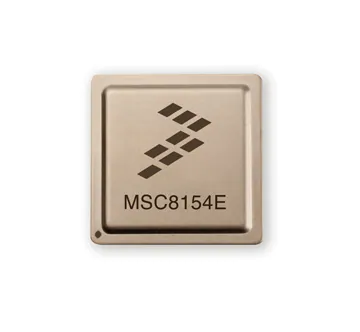
\includegraphics[scale=1]{images/MSC8154E_PRDIMG.png}}
\newcommand{\curso}{2021-2022}
\newcommand{\autor}{Jorge Benavides Macías \\ 05306948-C}
\begin{document}
%%%%%%%%%%%%%%%%%%%%%%%%%%%%%%%%%%%%%%%%%%%%%%%%%%%%%%%%%%%%%%%%%%%%%%%%
% Plantilla TFG/TFM
% Escuela Politécnica Superior de la Universidad de Alicante
% Realizado por: Jose Manuel Requena Plens
% Contacto: info@jmrplens.com / Telegram:@jmrplens
%%%%%%%%%%%%%%%%%%%%%%%%%%%%%%%%%%%%%%%%%%%%%%%%%%%%%%%%%%%%%%%%%%%%%%%%


\begin{titlepage}

% Márgenes de esta pagina modificados
\newgeometry{ignoreall,top=2cm,bottom=2cm}
\setlength{\centeroffset}{-0.5\oddsidemargin}
\addtolength{\centeroffset}{0.5\evensidemargin}
\thispagestyle{empty}

\AddToShipoutPictureBG*{%
\begin{tikzpicture}[overlay,remember picture]
\draw[line width=10pt]
    ($ (current page.north west) + (2cm,-2cm) $)
    rectangle
    ($ (current page.south east) + (-2cm,2cm) $);
\draw[line width=1.5pt]
    ($ (current page.north west) + (2.2cm,-2.2cm) $)
    rectangle
    ($ (current page.south east) + (-2.2cm,2.2cm) $);
\end{tikzpicture}
}

\FuenteTitulo
\centering
\vspace*{5em}
{\fontsize{30pt}{0pt}\selectfont \seguridadx}
\vfill
{\fontsize{25pt}{0pt}\selectfont \identificadorx}
\vfill
{\fontsize{25pt}{0pt}\selectfont \organizacionx}
\vfill
{\fontsize{25pt}{0pt}\selectfont \ul\titulox}
\vfill
% {\fontsize{20pt}{0pt}\selectfont \subtitulox}
% \vfill
{\fontsize{20pt}{0pt}\selectfont \autorx}

\vspace{1em}
{\fontsize{15pt}{0pt}\selectfont \asociacionx}
\vfill
{\fontsize{10pt}{0pt}\selectfont \fechax}
\vfill
{\fontsize{25pt}{0pt}\selectfont \tipox}
\vfill
{\fontsize{30pt}{0pt}\selectfont \seguridadx}
\vspace*{5em}
\vfill

% \def\FuenteTamano{50pt}
% % Titulo y subtitulo
% \vspace*{5em}
% \def\FuenteTamano{30pt}
% {\FuenteTitulo\fontsize{\FuenteTamano}{0pt}\selectfont\color{black} \seguridadx}
% \vfill
% \def\FuenteTamano{25pt}
% {\FuenteTitulo\fontsize{\FuenteTamano}{0pt}\selectfont\color{black} \identificadorx}
% \vfill
% {\FuentePortada \fontsize{\TamTrabajo}{35pt}\selectfont\color{black}\organizacionx}
% \vfill
% {\raggedright{\FuenteTitulo\fontsize{\FuenteTamano}{35pt}\selectfont\color{black} \titulox}}
% \vfill
% % {\raggedright{\FuenteTitulo\fontsize{\FuenteTamano}{110pt}\selectfont\color{black} \subtitulox }}
% % \vfill
% {\FuentePortada \fontsize{\TamTrabajo}{25pt}\selectfont\color{black} \autorx}
% \vfill
% {\FuentePortada \fontsize{\TamOtros}{30pt}\selectfont\color{black}\fechax}
% \vfill
% {\FuentePortada \fontsize{\TamTrabajo}{30pt}\selectfont\color{black}\tipox}
% \vfill
% \def\FuenteTamano{30pt}
% {\FuenteTitulo\fontsize{\FuenteTamano}{0pt}\selectfont\color{black} \seguridadx}
% \vspace{2cm}
% \vfill
\end{titlepage}

% A partir de aquí aplica los márgenes establecidos en configuracioninicial.tex
\restoregeometry

El dispositivo MSC8454E es un DSP de gama alta enfocado en las comunicaciones inalámbricas, se puede programar en C/C++ o en ensamblador. Como se observa en la figura \ref{fig:diagram_block} el núcleo del DSP tiene varios bloques de caché o memoria lo cual indica una arquitectura Harvard, cuenta con los periféricos de comunicación I2C, UART, IO y Clocks vistos en clase, además tiene algunos extra que dotan de distintas funcionalidades al dispositivo. 

Me gustaría destacar que cuenta con un subsistema que incluye un procesador RISC dual, independiente, que procesa las conexiones de dos puertos Ethernet y un SPI, me parece interesante ya que esto le da un nuevo uso a los DSP que no se me había ocurrido antes, la utilización de DSPs en módems o como se especifica en el párrafo inicial en comunicaciones inalámbricas que generalmente se asocian a Bluetooth o Wifi; también cuenta con dos controladores DDR lo cual es útil cuando se necesita leer o almacenar datos muy grandes. 

\begin{figure}[H]
    \centering
    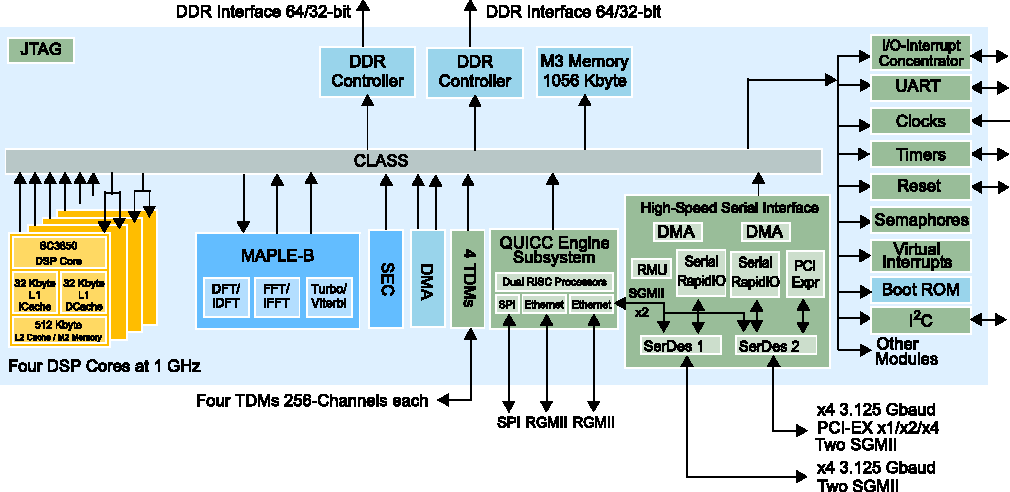
\includegraphics[scale=0.8]{images/diagram_block.pdf}
    \caption{Diagrama de bloques del DSP}
    \label{fig:diagram_block}
\end{figure}

{\Large \textbf{Interrupt Handling}}

Cuenta con un sistema de interrupciones internas y externas, además cuenta con la capacidad de emitir interrupciones a dispositivos externos; para las interrupciones externas hay 222 disponibles que se pueden configurar como enmascarables o no, como detalle más importante las interrupciones pueden ser tanto asíncronas como síncronas. Hay 3 niveles de gestión de interrupciones y cada una tiene características distintas.
\begin{itemize}
    \item \textbf{Interrupciones globales}
    
    Permite la generación de interrupciones virtuales, interrupciones virtuales no enmascarables que van a los núcleos e interrupciones a dispositivos externos.
    \item \textbf{Interrupciones generales}
    
    Dirige las interrupciones raras al núcleo.
    \item \textbf{Controlador de interrupción programable integrado (EPIC).}
    
    Asocia las interrupciones a un núcleo teniendo en cuenta la prioridad de las interrupciones. Cuenta con 256 interrupciones, incluyendo fuentes internas. 
\end{itemize}

La gestión de las interrupciones, dentro del dispositivo, cuenta con un sistema basado en niveles, dónde la fuente que genera la interrupción y como llega esta señal al núcleo son lo que generan la clasificación. 

Este sistema es más eficiente porque las interrupciones generadas dentro del núcleo son mucho más rápidas que las que puede generar el puerto UART o el IO ya que la interrupción pasa por otros bloques como el ``bloque general de configuración'' y la señal indirectamente se retrasa generando prioridades, además hay un bloque de registros que almacena estas señales de tal manera que siempre se procesan con prioridad. 

Este sistema queda reflejado en la siguiente figura.

\begin{figure}[H]
    \centering
    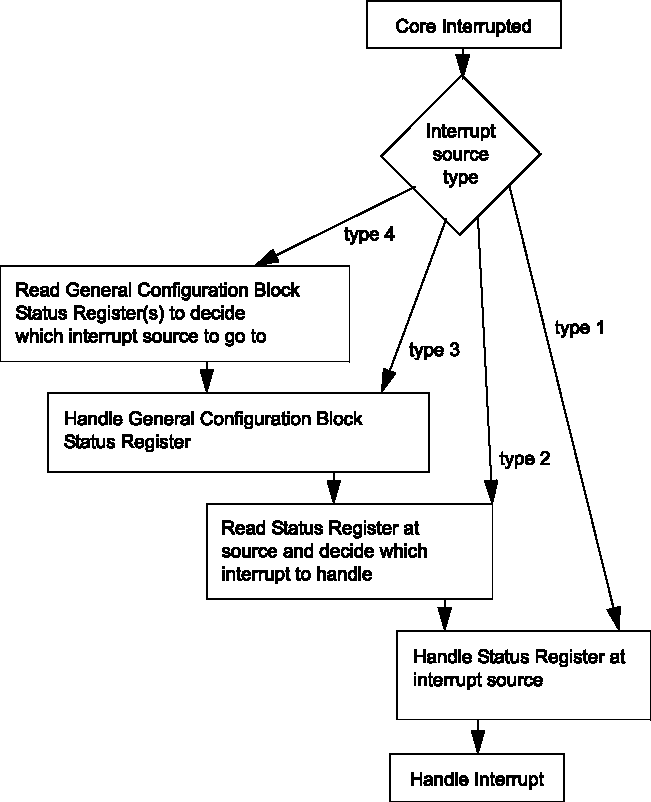
\includegraphics[scale=0.85]{images/diagram_flow.pdf}
    \caption{Flujo de gestión de interrupciones}
    \label{fig:interrupt_handling_flow}
\end{figure}

{\Large \textbf{Clocks}}

Este modelo de DPS cuenta con 5 PLLs (phase-locked loop).

Dos ellos tiene como objetivos sincronizar los relojes usados en el SerDes, un conjunto de bloques usados para pasar información de serie a paralelo y viceversa, la transmisión es a alta velocidad y se usa en el HSSI (una interfaz de transmisión serie a alta velocidad).

Los otros 3 PLLs tienen un uso genérico que se distribuye por todo el dispositivo, para controlar buses internos, subsistemas del núcleo, subsistemas generales, la memoria tanto caché como RAM e interfaces entrada/salida.

Es normal que con el aumento de la complejidad del dispositivo y las velocidades con las que se trabaja se precisen de tantos PLLs, incluso en versiones actuales la cantidad debe ser mucho mayor, puesto que el reloj tiene que distribuirse por muchas más zonas y pasar por más dispositivos el posible desfase que puede generarse es un problema bastante importante que requiere de nuevas topologías y dispositivos controladores para evitarlo.

{\Large \textbf{Hardware Semaphores}}

Es una variable de tipo abstracto que permite el acceso a recursos compartidos de múltiples procesos, es útil en la programación paralela o multihilo. Este dispositivo cuenta con 8 semáforos y como se observa en la figura \ref{fig:hardware_semaphoresl} los buses son de 8 bits por lo tanto usan una codificación parecida a la ``one-hot'', cuyo nombre es ``one-lock'', el cero representa que no está bloqueado, y el resto de combinaciones posibles, el one-lock se caracteriza porque una vez que está bloqueado, dicho bloqueo no puede cambiarse por otro, a menos que pase a estar libre.

\begin{figure}[H]
    \centering
    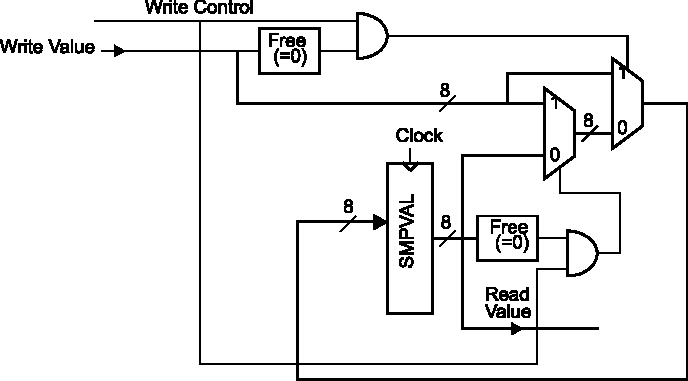
\includegraphics{images/hardware_semaphores.pdf}
    \caption{Diagramas de bloques del Hardware Semaphores.}
    \label{fig:hardware_semaphoresl}
\end{figure}

\fontsize{7.5}{1.2}\selectfont
\nocite{*}
\bibliographystyle{IEEEtran}
\bibliography{references}
\end{document}